\section{Proof for rank 5}


\subsection{Basic results}

\paragraph{}
Des lemmes qui semblent vrais et qui simplifierait grandement les preuves ci-dessous.

\begin{lemma}
  Si on a un carré alterné dont les indices différentes de 2 ou plus alors le seul moyen de l'étendre est d'utiliser un autre carré alterné.
\end{lemma}

\begin{corollary}
  Si nous travaillons sur un nombre impair de points et si nous avons un carré alterné dont la différence des indices est au moins 2, alors il existe un carré alterné dont la différence des indices est 1 parmi les "carrés alternés connexes".
\end{corollary}

\begin{proof}
  Chaque fois que nous étendons avec un carré alterné nous ajoutons deux points. Si nous avons un nombre impair de points alors nous ne pouvons pas utiliser que des carrés alternés pour les relier. Mais si nous avons un carré alterné dont la différence des indices est deux, nous devons forcément l'étendre à un autre carré alterné. Et ainsi de suite jusqu'à avoir tous les points ou à arriver à un carré alterné dont la différence des indice ne vaut plus qu'un. Le premier cas est impossible donc c'est forcément le second qui arriver.
\end{proof}

\begin{lemma}
  Une arête double dont la différence des indices est supérieur à 2 ne peut être relié que par un carré alterné.
\end{lemma}

\subsection{Intermediate results}

\begin{lemma}
  Dans un graphe CPR de rang 5 avec 11 points, il est impossible d'avoir un carré alterné entre $\rho_0$ et $\rho_4$ si $\rho_0$ est une 4-transposition\footnote{Cette dernière condition est-elle nécessaire?}
\end{lemma}

\begin{proof}
  Commençons par placer l'involution $\rho_0$ sur le graphe. Le graphe est toujours composé de 4 arêtes isolées donc, à un isomorphisme près, on a le graphe suivant:

  \begin{figure}[H]
    \begin{center}
      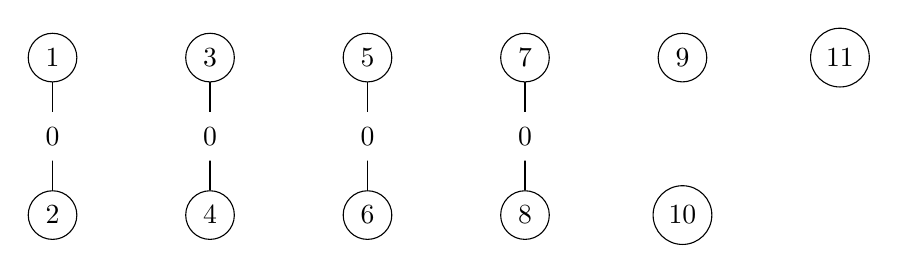
\begin{tikzpicture}

        \begin{scope}[every node/.style={circle,draw}]
          \node (1)  at (0,2)  {1};
          \node (2)  at (0,0)  {2};
          \node (3)  at (2,2)  {3};
          \node (4)  at (2,0)  {4};
          \node (5)  at (4,2)  {5};
          \node (6)  at (4,0)  {6};
          \node (7)  at (6,2)  {7};
          \node (8)  at (6,0)  {8};
          \node (9)  at (8,2)  {9};
          \node (10) at (8,0)  {10};
          \node (11) at (10,2) {11};
        \end{scope}

        \begin{scope}[every node/.style={fill=white,circle}]

          \begin{scope}[every edge/.style={draw}]
            \path (1)  edge node {$0$} (2);
            \path (3)  edge node {$0$} (4);
            \path (5)  edge node {$0$} (6);
            \path (7)  edge node {$0$} (8);
          \end{scope}
        \end{scope}

      \end{tikzpicture}
      \caption{$\rho_0$ est une 4-transposition}
    \end{center}
  \end{figure}

  \paragraph{}
  Maitenant plaçons un carré alterné entre $\rho_0$ et $\rho_4$.

  \begin{figure}[H]
    \begin{center}
      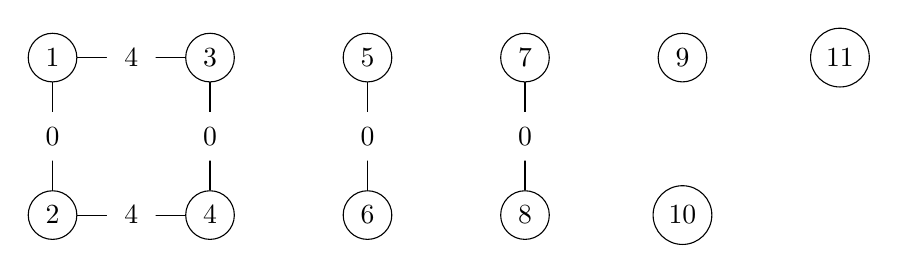
\begin{tikzpicture}

        \begin{scope}[every node/.style={circle,draw}]
          \node (1)  at (0,2)  {1};
          \node (2)  at (0,0)  {2};
          \node (3)  at (2,2)  {3};
          \node (4)  at (2,0)  {4};
          \node (5)  at (4,2)  {5};
          \node (6)  at (4,0)  {6};
          \node (7)  at (6,2)  {7};
          \node (8)  at (6,0)  {8};
          \node (9)  at (8,2)  {9};
          \node (10) at (8,0)  {10};
          \node (11) at (10,2) {11};
        \end{scope}

        \begin{scope}[every node/.style={fill=white,circle}]

          \begin{scope}[every edge/.style={draw}]
            \path (1)  edge node {$0$} (2);
            \path (3)  edge node {$0$} (4);
            \path (5)  edge node {$0$} (6);
            \path (7)  edge node {$0$} (8);
            \path (1)  edge node {$4$} (3);
            \path (2)  edge node {$4$} (4);
          \end{scope}
        \end{scope}

      \end{tikzpicture}
      \caption{Cas 1: carré alterné}
    \end{center}
  \end{figure}

  \paragraph{}
  Par le lemme précédent, on doit trouver une suite de carré alternés jusqu'à ce que la différence ne soit que deux. En partant du carré $(0,4)$, on doit avoir au moins 3 carrés pour satisfaire cette contrainte. Il est possible de le faire avec 5 carrés mais il faudrait 12 points ce que nous n'avons pas.

  \paragraph{}
  En partant du carré $(0,4)$ on peut aller au carré $(1,4)$ ou au carré $(0,3)$. Mais si nous n'utilisons pas les involutions $\rho_0$ maintenant, nous ne pourrons jamais les utiliser plus loin dans les carrés alternés. Les deux arêtes isolées occupent 4 points et le carré que nous formons va en utiliser 8, donc il faut que nous utilisions au moins une de ces arêtes sinon nous n'aurons pas assez de points. La carré suivant est donc $(0,3)$.

  \paragraph{}
  Ensuite nous avons le choix entre $(0,2)$ et $(1,3)$. Le second choix est impossible, en effet la suite de carrés alternés occupent 8 points et ne peut être reliée que par des arêtes $\rho_2$. Mais nous n'avons utilisé qu'une arête $\rho_3$, il en faut donc une seconde mais celle-ci ne peut pas toucher les carrés alternés. De l'autre côté nous avons l'arête $\rho_1$ isolée mais la seconde arête ne peut pas former de carré alterné avec celle-ci. Il faut donc qu'elle double l'arête $\rho_0$ mais une arête double $(0,3)$ ne peut être reliée que par un carré alterné mais il n'y a plus assez de points. Le troisième carré est donc $(0,2)$, pour connecter ce carré, nous sommes obligés d'utiliser une arête $\rho_1$ ce qui nous donne le graphe suivant:


  \begin{figure}[H]
    \begin{center}
      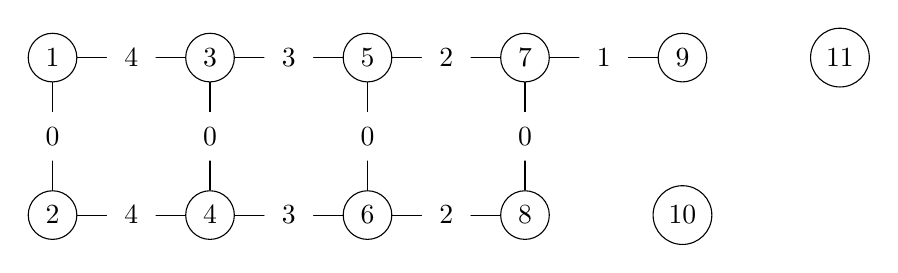
\begin{tikzpicture}

        \begin{scope}[every node/.style={circle,draw}]
          \node (1)  at (0,2)  {1};
          \node (2)  at (0,0)  {2};
          \node (3)  at (2,2)  {3};
          \node (4)  at (2,0)  {4};
          \node (5)  at (4,2)  {5};
          \node (6)  at (4,0)  {6};
          \node (7)  at (6,2)  {7};
          \node (8)  at (6,0)  {8};
          \node (9)  at (8,2)  {9};
          \node (10) at (8,0)  {10};
          \node (11) at (10,2) {11};
        \end{scope}

        \begin{scope}[every node/.style={fill=white,circle}]

          \begin{scope}[every edge/.style={draw}]
            \path (1)  edge node {$0$} (2);
            \path (3)  edge node {$0$} (4);
            \path (5)  edge node {$0$} (6);
            \path (7)  edge node {$0$} (8);
            \path (7)  edge node {$1$} (9);
            \path (5)  edge node {$2$} (7);
            \path (6)  edge node {$2$} (8);
            \path (3)  edge node {$3$} (5);
            \path (4)  edge node {$3$} (6);
            \path (1)  edge node {$4$} (3);
            \path (2)  edge node {$4$} (4);
          \end{scope}
        \end{scope}

      \end{tikzpicture}
      \caption{Cas 1.1: doubles carrés alternés}
    \end{center}
  \end{figure}

  \paragraph{}
  Pour relier les deux derniers points, uniquement 2 arêtes sont nécessaires mais alors le nombre total d'arêtes serait impair ce qui interdit. Il faut donc former un carré alterné ou une arête double. Le carré alterné est impossible car le nombre de points est insuffisant. Il faut donc utiliser une arête double avec exactement 2 de différence. Toutes les arêtes $\rho_0$ on déjà été utilisées, les seules possibilités sont une arête double $(1,3)$ ou une arête double $(2,4)$ mais dans les deux cas soit le nombre d'arêtes $\rho_3$ soit $\rho_4$ devient impair. Donc c'est impossible.
\end{proof}

\subsection{Main theorems}

\begin{lemma}
  $\rho_0$ (et donc $\rho_4$) ne peut être une 4-transposition.
\end{lemma}

\begin{proof}
  Considérons maintenant l'autre cas qui contient une arête double $(0,4)$. Nous partons donc du graphe suivant.

  \paragraph{}
  Il faut maintenant placer $\rho_3$ tel qu'il commute avec $\rho_0$ mais ni avec $\rho_2$ et $\rho_4$. Nous avons trois possibilités, nous pouvons former un carré alterné avec $\rho_0$, double des arêtes $\rho_0$ mais sans former de carré alterné avec $\rho_2$ et $\rho_4$ ou alors double une arête et relier deux points encore fixes.

  \begin{figure}[H]
    \begin{center}
      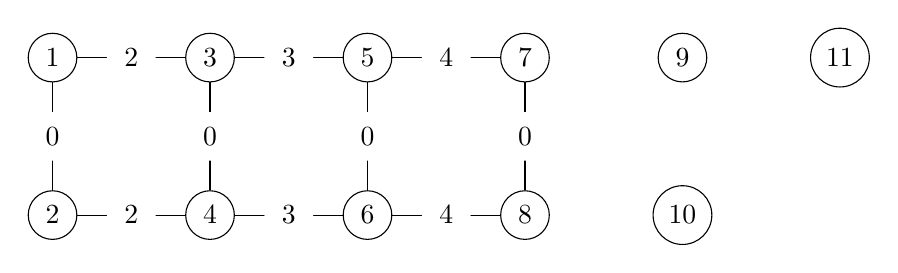
\begin{tikzpicture}

        \begin{scope}[every node/.style={circle,draw}]
          \node (1)  at (0,2)  {1};
          \node (2)  at (0,0)  {2};
          \node (3)  at (2,2)  {3};
          \node (4)  at (2,0)  {4};
          \node (5)  at (4,2)  {5};
          \node (6)  at (4,0)  {6};
          \node (7)  at (6,2)  {7};
          \node (8)  at (6,0)  {8};
          \node (9)  at (8,2)  {9};
          \node (10) at (8,0)  {10};
          \node (11) at (10,2) {11};
        \end{scope}

        \begin{scope}[every node/.style={fill=white,circle}]

          \begin{scope}[every edge/.style={draw}]
            \path (1)  edge node {$0$} (2);
            \path (3)  edge node {$0$} (4);
            \path (5)  edge node {$0$} (6);
            \path (7)  edge node {$0$} (8);
            \path (1)  edge node {$2$} (3);
            \path (2)  edge node {$2$} (4);
            \path (3)  edge node {$3$} (5);
            \path (4)  edge node {$3$} (6);
            \path (5)  edge node {$4$} (7);
            \path (6)  edge node {$4$} (8);
          \end{scope}
        \end{scope}

      \end{tikzpicture}
      \caption{Cas 1.1.1: triples carrés alternés}
    \end{center}
  \end{figure}

  Maintenant il faut placer $\rho_1$ qui doit être une 4-transposition car sinon on n'a pas assez d'arêtes pour terminer. Mais on a que deux point d'accroche sur le graphe actuel donc c'est impossible.

  \begin{figure}[H]
    \begin{center}
      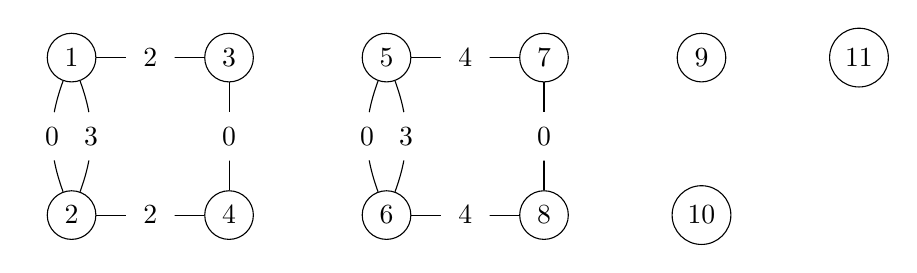
\begin{tikzpicture}

        \begin{scope}[every node/.style={circle,draw}]
          \node (1)  at (0,2)  {1};
          \node (2)  at (0,0)  {2};
          \node (3)  at (2,2)  {3};
          \node (4)  at (2,0)  {4};
          \node (5)  at (4,2)  {5};
          \node (6)  at (4,0)  {6};
          \node (7)  at (6,2)  {7};
          \node (8)  at (6,0)  {8};
          \node (9)  at (8,2)  {9};
          \node (10) at (8,0)  {10};
          \node (11) at (10,2) {11};
        \end{scope}

        \begin{scope}[every node/.style={fill=white,circle}]

          \begin{scope}[every edge/.style={draw}]
            \path (1)  edge[bend right=20] node {$0$} (2);
            \path (3)  edge node {$0$} (4);
            \path (5)  edge[bend right=20] node {$0$} (6);
            \path (7)  edge node {$0$} (8);
            \path (1)  edge node {$2$} (3);
            \path (2)  edge node {$2$} (4);
            \path (1)  edge[bend left=20] node {$3$} (2);
            \path (5)  edge[bend left=20] node {$3$} (6);
            \path (5)  edge node {$4$} (7);
            \path (6)  edge node {$4$} (8);
          \end{scope}
        \end{scope}

      \end{tikzpicture}
      \caption{Cas 1.1.2: doubles carrés alternés et arêtes doublées}
    \end{center}
  \end{figure}

  Içi aussi $\rho_1$ doit être une 4-transposition mais nous n'avons encore que 2 points d'attache.

  Maintenant il faut placer $\rho_1$ qui doit être une 4-transposition car sinon on n'a pas assez d'arêtes pour terminer. Mais on a que deux point d'accroche sur le graphe actuel donc c'est impossible.

  \begin{figure}[H]
    \begin{center}
      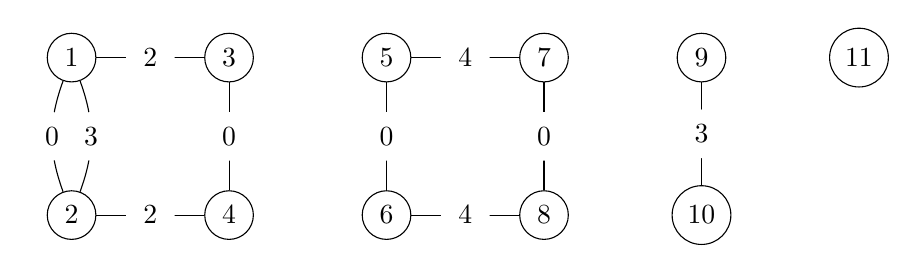
\begin{tikzpicture}

        \begin{scope}[every node/.style={circle,draw}]
          \node (1)  at (0,2)  {1};
          \node (2)  at (0,0)  {2};
          \node (3)  at (2,2)  {3};
          \node (4)  at (2,0)  {4};
          \node (5)  at (4,2)  {5};
          \node (6)  at (4,0)  {6};
          \node (7)  at (6,2)  {7};
          \node (8)  at (6,0)  {8};
          \node (9)  at (8,2)  {9};
          \node (10) at (8,0)  {10};
          \node (11) at (10,2) {11};
        \end{scope}

        \begin{scope}[every node/.style={fill=white,circle}]

          \begin{scope}[every edge/.style={draw}]
            \path (1)  edge[bend right=20] node {$0$} (2);
            \path (3)  edge node {$0$} (4);
            \path (5)  edge node {$0$} (6);
            \path (7)  edge node {$0$} (8);
            \path (1)  edge node {$2$} (3);
            \path (2)  edge node {$2$} (4);
            \path (1)  edge[bend left=20] node {$3$} (2);
            \path (9)  edge node {$3$} (10);
            \path (5)  edge node {$4$} (7);
            \path (6)  edge node {$4$} (8);
          \end{scope}
        \end{scope}

      \end{tikzpicture}
      \caption{Cas 1.1.3: doubles carrés alternés, une arête doublée avec $\rho_2$}
    \end{center}
  \end{figure}

  Ici nous devons utiliser $\rho_1$ pour former une carré alterné pour relier les deux composantes de gauche, mais nous devonc aussi en utiliser un pour attcher l'arête $\rho_3$ isolée. Mais nous avons utilisé toutes nos arêtes et le point 11 n'est toujours pas relié.

  \begin{figure}[H]
    \begin{center}
      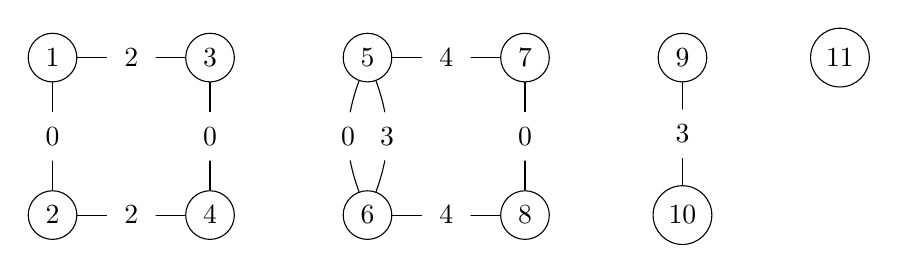
\begin{tikzpicture}

        \begin{scope}[every node/.style={circle,draw}]
          \node (1)  at (0,2)  {1};
          \node (2)  at (0,0)  {2};
          \node (3)  at (2,2)  {3};
          \node (4)  at (2,0)  {4};
          \node (5)  at (4,2)  {5};
          \node (6)  at (4,0)  {6};
          \node (7)  at (6,2)  {7};
          \node (8)  at (6,0)  {8};
          \node (9)  at (8,2)  {9};
          \node (10) at (8,0)  {10};
          \node (11) at (10,2) {11};
        \end{scope}

        \begin{scope}[every node/.style={fill=white,circle}]

          \begin{scope}[every edge/.style={draw}]
            \path (1)  edge node {$0$} (2);
            \path (3)  edge node {$0$} (4);
            \path (5)  edge[bend right=20] node {$0$} (6);
            \path (7)  edge node {$0$} (8);
            \path (1)  edge node {$2$} (3);
            \path (2)  edge node {$2$} (4);
            \path (5)  edge[bend left=20] node {$3$} (6);
            \path (9)  edge node {$3$} (10);
            \path (5)  edge node {$4$} (7);
            \path (6)  edge node {$4$} (8);
          \end{scope}
        \end{scope}

      \end{tikzpicture}
      \caption{Cas 1.1.4: doubles carrés alternés, une arête doublée avec $\rho_4$}
    \end{center}
  \end{figure}

  \paragraph{}
  Ici, l'arête isolée $\rho_3$ ne pourra jamais être reliée uniquement avec des arêtes $\rho_1$, en effet il faut former un carré alterné avec l'autre arête $\rho_3$ mais un carré alterné n'est pas possible à cet endroit à cause des arêtes $\rho_4$ adjacentes.

  \paragraph{}
  L'idée de placer $\rho_4$ pour former des carrés alternés est mauvaise, essayons donc de doubler des arêtes de $\rho_0$.

  \begin{figure}[H]
    \begin{center}
      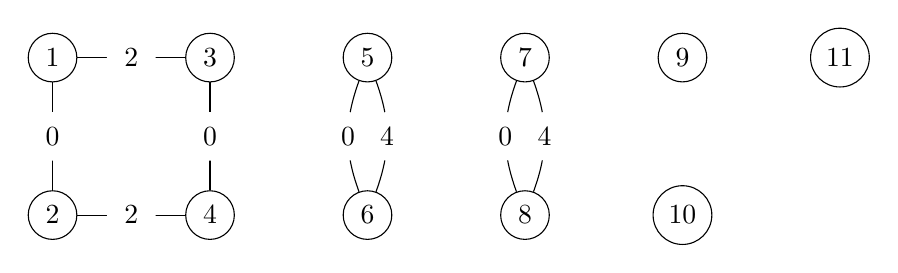
\begin{tikzpicture}

        \begin{scope}[every node/.style={circle,draw}]
          \node (1)  at (0,2)  {1};
          \node (2)  at (0,0)  {2};
          \node (3)  at (2,2)  {3};
          \node (4)  at (2,0)  {4};
          \node (5)  at (4,2)  {5};
          \node (6)  at (4,0)  {6};
          \node (7)  at (6,2)  {7};
          \node (8)  at (6,0)  {8};
          \node (9)  at (8,2)  {9};
          \node (10) at (8,0)  {10};
          \node (11) at (10,2) {11};
        \end{scope}

        \begin{scope}[every node/.style={fill=white,circle}]

          \begin{scope}[every edge/.style={draw}]
            \path (1)  edge node {$0$} (2);
            \path (3)  edge node {$0$} (4);
            \path (5)  edge[bend right=20] node {$0$} (6);
            \path (7)  edge[bend right=20] node {$0$} (8);
            \path (1)  edge node {$2$} (3);
            \path (2)  edge node {$2$} (4);
            \path (5)  edge[bend left=20] node {$4$} (6);
            \path (7)  edge[bend left=20] node {$4$} (8);
          \end{scope}
        \end{scope}

      \end{tikzpicture}
      \caption{Cas 1.2: carré alterné et arêtes doublées}
    \end{center}
  \end{figure}


\end{proof}

\begin{theorem}
  Si $\rho_1$ (ou $\rho_3$) est une 4-transposition alors $\rho_2$ l'est aussi.
\end{theorem}

\begin{proof}
  Supposons que $\rho_1$ soit une 4-transposition, elle doit commuter avec $\rho_3$ et $\rho_4$. $\rho_4$ peut soit former un carré alterné, soit doubler deux arêtes, soit doubler une arête et relier deux points encore fixes.

  \paragraph{}
  Si $\rho_4$ forme un carré alterné avec $\rho_1$, il doit être adjacent à un carré alterné entre $\rho_3$ et $\rho_1$ ($\rho_2$ et $\rho_4$ n'est pas envisageable car $\rho_4$ est une 2-transposition). On se trouve donc avec le graphe suivant:

  \begin{figure}[H]
    \begin{center}
      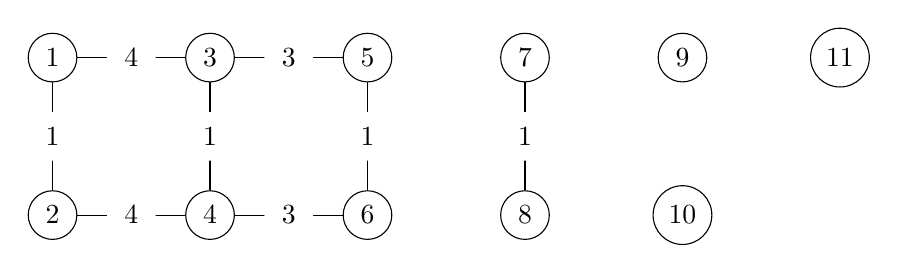
\begin{tikzpicture}

        \begin{scope}[every node/.style={circle,draw}]
          \node (1)  at (0,2)  {1};
          \node (2)  at (0,0)  {2};
          \node (3)  at (2,2)  {3};
          \node (4)  at (2,0)  {4};
          \node (5)  at (4,2)  {5};
          \node (6)  at (4,0)  {6};
          \node (7)  at (6,2)  {7};
          \node (8)  at (6,0)  {8};
          \node (9)  at (8,2)  {9};
          \node (10) at (8,0)  {10};
          \node (11) at (10,2) {11};
        \end{scope}

        \begin{scope}[every node/.style={fill=white,circle}]

          \begin{scope}[every edge/.style={draw}]
            \path (1)  edge node {$1$} (2);
            \path (3)  edge node {$1$} (4);
            \path (5)  edge node {$1$} (6);
            \path (7)  edge node {$1$} (8);
            \path (3)  edge node {$3$} (5);
            \path (4)  edge node {$3$} (6);
            \path (1)  edge node {$4$} (3);
            \path (2)  edge node {$4$} (4);
          \end{scope}
        \end{scope}

      \end{tikzpicture}
      \caption{Un carré alterné et son voisin engendré}
    \end{center}
  \end{figure}

  \paragraph{}
  Maintenant si nous essayons de placer les arêtes $\rho_0$, nous avons un problème car nous n'avons qu'une arête $\rho_1$ pour les relier au reste. Il faut donc former un carré alterné entre $\rho_0$ et $\rho_2$ et relier ce carré au reste grâce à l'arête $\rho_1$. On a le graphe suivant.
  % TODO une petite preuve ?

  \begin{figure}[H]
    \begin{center}
      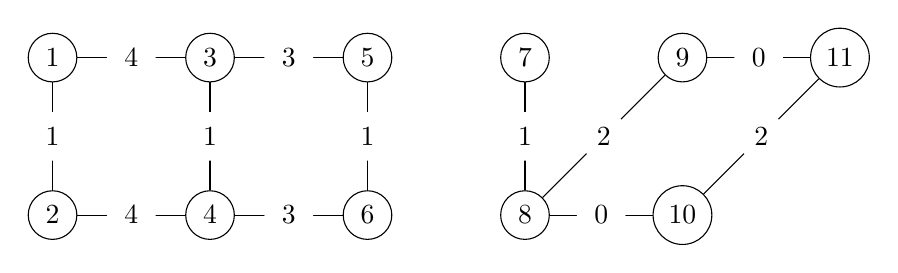
\begin{tikzpicture}

        \begin{scope}[every node/.style={circle,draw}]
          \node (1)  at (0,2)  {1};
          \node (2)  at (0,0)  {2};
          \node (3)  at (2,2)  {3};
          \node (4)  at (2,0)  {4};
          \node (5)  at (4,2)  {5};
          \node (6)  at (4,0)  {6};
          \node (7)  at (6,2)  {7};
          \node (8)  at (6,0)  {8};
          \node (9)  at (8,2)  {9};
          \node (10) at (8,0)  {10};
          \node (11) at (10,2) {11};
        \end{scope}

        \begin{scope}[every node/.style={fill=white,circle}]

          \begin{scope}[every edge/.style={draw}]
            \path (9)  edge node {$0$} (11);
            \path (8)  edge node {$0$} (10);
            \path (1)  edge node {$1$} (2);
            \path (3)  edge node {$1$} (4);
            \path (5)  edge node {$1$} (6);
            \path (7)  edge node {$1$} (8);
            \path (8)  edge node {$2$} (9);
            \path (10) edge node {$2$} (11);
            \path (3)  edge node {$3$} (5);
            \path (4)  edge node {$3$} (6);
            \path (1)  edge node {$4$} (3);
            \path (2)  edge node {$4$} (4);
          \end{scope}
        \end{scope}

      \end{tikzpicture}
      \caption{Un carré alterné et son voisin engendré}
    \end{center}
  \end{figure}

  \paragraph{}
  Pour compléter le graphe, il faut encore utiliser 2 arêtes $\rho_2$. Il n'est pas possible d'utilise deux arêtes $\rho_3$ supplémentaires. % TODO Pourquoi ?

  \paragraph{}
  Maintenant il faut placer les arêtes $\rho_3$, nous avons deux possibilités, soit $\rho_3$ est une 2-transposition, soit il s'agit d'une 4-transposition. Si c'est un 2-transposition, tout est déjà placé. De plus nous avons déjà placé deux arêtes non-essentielles. Il est impossible de compléter le graphe sans utiliser au moins une autre arête non-essentielle. En effet, si nous continuons le graphe, nous pouvons connecter jusqu'à deux arêtes $\rho_2$. Plaçons-en une, si nous voulons continuer, nous devons maintenant utiliser l'arête $\rho_1$ isolée, suivie par une arête $\rho_0$. Mais nous n'avons aucune façon de placer la dernière arête $\rho_0$.

  \paragraph{}
  Il faut donc au moins trois arêtes non-essentielles mais alors il faut au moins deux 4-transpositions qui sont forcément $\rho_1$ et $\rho_2$.

  \paragraph{}
  Étudions maintenant le cas où $\rho_3$ est une 4-transposition. Il reste alors 2 arêtes $\rho_3$ à placer.

  \paragraph{}
  Pour $\rho_4$, s'il forme un carré avec $\rho_1$, on ne pourra le relier avec rien car il y deux involutions entre $\rho_1$ et $\rho_4$ et non une. Si par contre $\rho_4$ double un arête et relie deux points fixes. Alors ces deux points nouvellement reliés ne pourront jamais être reliés au reste du graphe car l'involution $\rho_3$ forme un carré alterné et n'est donc pas disponible.
\end{proof}

\begin{theorem}
  Soit un sggi de rang 5 sur $A_{11}$. Alors ce sggi contient exactement une 4-transposition.
\end{theorem}

Il nous reste deux cas à analyser, celui où il y a deux 4-transpositions, celles-ci sont alors forcément en $\rho_1$ et $\rho_2$ (à la dualité près) et celui où on a trois 4-transpositions qui sont alors positionnées en $\rho_1$, $\rho_2$ et $\rho_3$.

\begin{proof}
  En partant du graphe de la preuve précédente, si on rajoute l'involution $\rho_3$, on l'étend à $A_{11}$.
  En effet, partons du graphe et essayons de rajouter la 2-transposition $\rho_3$, celle-ci doit commuter avec $\rho_0$ et $\rho_1$.
  \begin{figure}[H]
    \begin{center}
      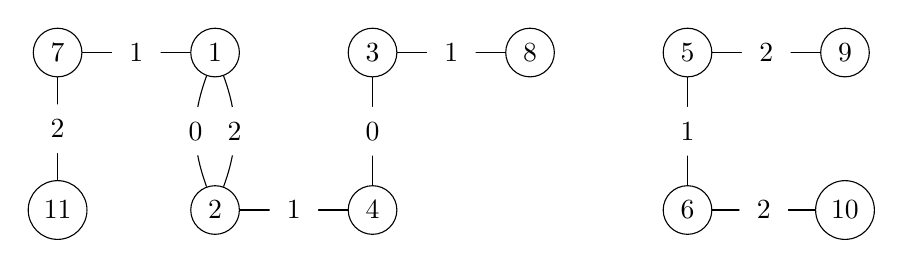
\begin{tikzpicture}

        \begin{scope}[every node/.style={circle,draw}]
          \node (1)  at (0,2)  {1};
          \node (2)  at (0,0)  {2};
          \node (3)  at (2,2)  {3};
          \node (4)  at (2,0)  {4};
          \node (5)  at (6,2)  {5};
          \node (6)  at (6,0)  {6};
          \node (7)  at (-2,2) {7};
          \node (8)  at (4,2)  {8};
          \node (9)  at (8,2)  {9};
          \node (10) at (8,0) {10};
          \node (11) at (-2,0) {11};
        \end{scope}

        \begin{scope}[every node/.style={fill=white,circle}]

          \begin{scope}[every edge/.style={draw}]
            \path (1)  edge[bend right=20] node {$0$} (2);
            \path (3)  edge node {$0$} (4);
            \path (1)  edge node {$1$} (7);
            \path (2)  edge node {$1$} (4);
            \path (3)  edge node {$1$} (8);
            \path (5)  edge node {$1$} (6);
            \path (1)  edge[bend left=20] node {$2$} (2);
            \path (5)  edge node {$2$} (9);
            \path (6)  edge node {$2$} (10);
            \path (7)  edge node {$2$} (11);
          \end{scope}
        \end{scope}

      \end{tikzpicture}
      \caption{Example of subgroup of sggi of type 2}
    \end{center}
  \end{figure}

  \paragraph{}
  Nous devons utiliser 2 arêtes $\rho_3$, pour cela nous avons trois possibilités, sachant que nous pouvons ignorer les arêtes $\rho_2$.
  \begin{enumerate}
    \item Relier deux points non reliés
    \item Doubler une arête
    \item Former un carré alterné
  \end{enumerate}

  \paragraph{}
  Dans la composante de gauche, suite à l'alternance des arêtes $\rho_0$ et $\rho_1$ il n'est pas possible de former un carré alterné ou une arête double, la seule possibilité est une arête qui partirait du point 11. Dans la composante de droite, les possibilités sont plus variés. On doit placer deux arêtes en tout et pour le moment nous n'avons trouvé qu'un point d'attache potentiel. Il en faut donc au moins 3 autres parmi les 4 points qui compose cette composante. Nous sommes donc obligé d'utiliser le point 5 ou le point 6 mais dans ce cas, nous sommes obligés de doubler l'arête $\rho_1$ présente à cet endroit. Pour la dernière arête soit nous relions les deux points restants dans la composante de droite soit nous relions un de ces points à l'autre composante.

  \paragraph{}
  Dans le premier cas nous ne pourrons jamais atteindre $A_{11}$. En effet, nous avons le graphe suivant
  \begin{figure}[H]
    \begin{center}
      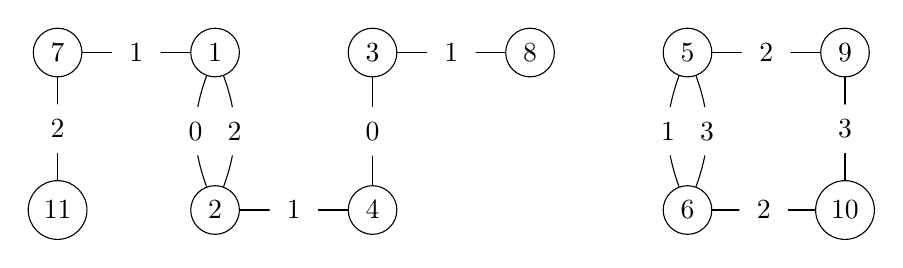
\begin{tikzpicture}

        \begin{scope}[every node/.style={circle,draw}]
          \node (1)  at (0,2)  {1};
          \node (2)  at (0,0)  {2};
          \node (3)  at (2,2)  {3};
          \node (4)  at (2,0)  {4};
          \node (5)  at (6,2)  {5};
          \node (6)  at (6,0)  {6};
          \node (7)  at (-2,2) {7};
          \node (8)  at (4,2)  {8};
          \node (9)  at (8,2)  {9};
          \node (10) at (8,0) {10};
          \node (11) at (-2,0) {11};
        \end{scope}

        \begin{scope}[every node/.style={fill=white,circle}]

          \begin{scope}[every edge/.style={draw}]
            \path (1)  edge[bend right=20] node {$0$} (2);
            \path (3)  edge node {$0$} (4);
            \path (1)  edge node {$1$} (7);
            \path (2)  edge node {$1$} (4);
            \path (3)  edge node {$1$} (8);
            \path (5)  edge[bend right=20] node {$1$} (6);
            \path (1)  edge[bend left=20] node {$2$} (2);
            \path (5)  edge node {$2$} (9);
            \path (6)  edge node {$2$} (10);
            \path (7)  edge node {$2$} (11);
            \path (5)  edge[bend left=20] node {$3$} (6);
            \path (9)  edge node {$3$} (10);
          \end{scope}
        \end{scope}

      \end{tikzpicture}
      \caption{Example of subgroup of sggi of type 2}
    \end{center}
  \end{figure}

  \paragraph{}
  Dans cet graphe, $\rho_2$ et $\rho_3$ commute donc ce graphe ne peut être celui d'un groupe semi-simple. Même si nous rajoutons des involutions, cela ne changera rien à ce résultat et le graphe ne pourra jamais être celui d'$A_{11}$. La seule possibilité qu'il nous reste est le premier graphe.

  \begin{figure}[H]
    \begin{center}
      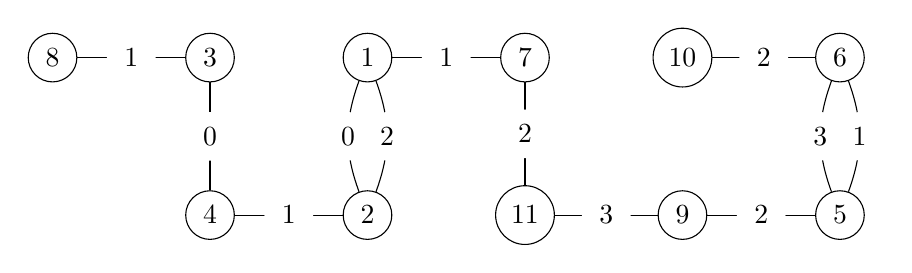
\begin{tikzpicture}

        \begin{scope}[every node/.style={circle,draw}]
          \node (1)  at (2,2)  {1};
          \node (2)  at (2,0)  {2};
          \node (3)  at (0,2)  {3};
          \node (4)  at (0,0)  {4};
          \node (5)  at (8,0)  {5};
          \node (6)  at (8,2)  {6};
          \node (7)  at (4,2) {7};
          \node (8)  at (-2,2)  {8};
          \node (9)  at (6,0)  {9};
          \node (10) at (6,2) {10};
          \node (11) at (4,0) {11};
        \end{scope}

        \begin{scope}[every node/.style={fill=white,circle}]

          \begin{scope}[every edge/.style={draw}]
            \path (1)  edge[bend right=20] node {$0$} (2);
            \path (3)  edge node {$0$} (4);
            \path (1)  edge node {$1$} (7);
            \path (2)  edge node {$1$} (4);
            \path (3)  edge node {$1$} (8);
            \path (5)  edge[bend right=20] node {$1$} (6);
            \path (1)  edge[bend left=20] node {$2$} (2);
            \path (5)  edge node {$2$} (9);
            \path (6)  edge node {$2$} (10);
            \path (7)  edge node {$2$} (11);
            \path (5)  edge[bend left=20] node {$3$} (6);
            \path (9)  edge node {$3$} (11);
          \end{scope}
        \end{scope}

      \end{tikzpicture}
      \caption{Example of subgroup of sggi of type 2}
    \end{center}
  \end{figure}

\end{proof}

\begin{lemma}
  Ce graphe engendre $A_{11}$.
\end{lemma}



\begin{theorem}
  Soit un sggi de rang 5 sur $A_{11}$. Alors ce sggi n'est pas un C-group.
\end{theorem}

\begin{proof}
  Partons d'un diagramme avec juste la 4-transposition.

  \begin{figure}[H]
    \begin{center}
      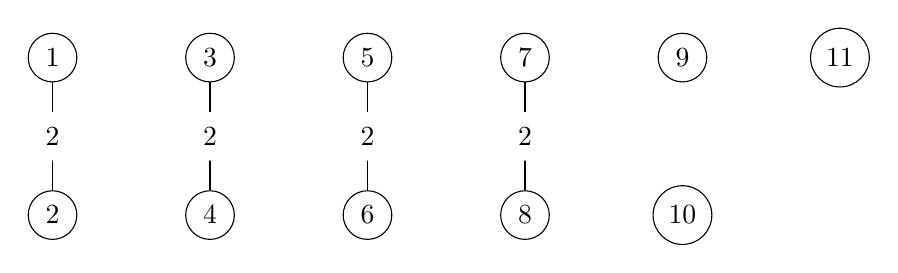
\begin{tikzpicture}

        \begin{scope}[every node/.style={circle,draw}]
          \node (1)  at (0,2)  {1};
          \node (2)  at (0,0)  {2};
          \node (3)  at (2,2)  {3};
          \node (4)  at (2,0)  {4};
          \node (5)  at (4,2)  {5};
          \node (6)  at (4,0)  {6};
          \node (7)  at (6,2)  {7};
          \node (8)  at (6,0)  {8};
          \node (9)  at (8,2)  {9};
          \node (10) at (8,0)  {10};
          \node (11) at (10,2) {11};
        \end{scope}

        \begin{scope}[every node/.style={fill=white,circle}]

          \begin{scope}[every edge/.style={draw}]
            \path (1)  edge node {$2$} (2);
            \path (3)  edge node {$2$} (4);
            \path (5)  edge node {$2$} (6);
            \path (7)  edge node {$2$} (8);
          \end{scope}
        \end{scope}

      \end{tikzpicture}
      \caption{[1, 5, 1010, 232, 381]}
    \end{center}
  \end{figure}

\paragraph{}
Nous allons essayer d'ajouter les involutions $\rho_0$ et $\rho_4$. Celles-ci doivent commuter avec $\rho_2$. Pour chaque involution nous devons choisir entre les 3 possibilités suivantes:
\begin{enumerate}
  \item Faire un arête double avec $\rho_2$ et reliés deux points qui sont, pour le moment, fixes.
  \item Faire deux arêtes doubles avec $\rho_2$.
  \item Faire un carré alterné avec $\rho_2$.
\end{enumerate}

\paragraph{}
S'il n'y a qu'une seule 4-transposition, alors nous avons 12 arêtes pour relier 11 points soit 2 de plus que le strict minimum. Sauf pour deux arêtes nous devons toujours relier deux composantes connexes différentes. Quand nous faisons un carré, nous utilisons une de ces deux arêtes et il se passe la même chose quand nous utilisons une arête double.

\paragraph{}
Nous ne pouvons jamais faire le second choix pour une involution car sinon nous aurions déjà utilisé nos deux arêtes et nous ne pourrions plus nous occuper de la seconde.

\paragraph{}
Remarquons qu'il est impossible de faire le même choix pour $\rho_0$ et $\rho_4$. Dans le premier cas, on aurait pas assez de point fixes. Dans le troisième cas, nous ne pouvons pas utiliser le même carré car cela formerait des arêtes doubles et donc il faudrait 3 arêtes libres. Il est impossible de faire deux carrés adjacents

\paragraph{}
Nous ne pouvons utiliser deux carrés adjacents car nous aurions une involution $\rho_0$ et $\rho_4$ adjacente mais nous avons déjà utilisé toutes les arêtes de ces involutions donc nous pouvons pas avoir un sggi.

\paragraph{}
Dans le cas deux deux carrés disjoints, nous ne pouvons pas les relier car il ne nous reste que des involutions $\rho_1$ et $\rho_3$ et celles-ce ne peuvent être adjacentes sans former un carré mais ça c'est impossible.

\paragraph{}
La seule possibilité qu'il nous reste est de choisir que $\rho_0$ reliera deux point fixes et doublera une arête et que $\rho_4$ formera un carré alterné. On a donc le graphe suivant.


\begin{figure}[H]
  \begin{center}
    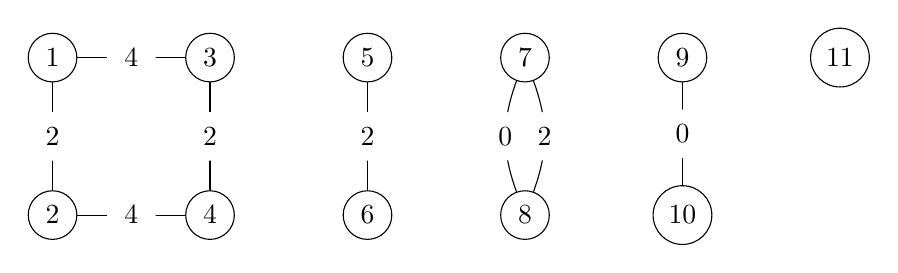
\begin{tikzpicture}

      \begin{scope}[every node/.style={circle,draw}]
        \node (1)  at (0,2)  {1};
        \node (2)  at (0,0)  {2};
        \node (3)  at (2,2)  {3};
        \node (4)  at (2,0)  {4};
        \node (5)  at (4,2)  {5};
        \node (6)  at (4,0)  {6};
        \node (7)  at (6,2)  {7};
        \node (8)  at (6,0)  {8};
        \node (9)  at (8,2)  {9};
        \node (10) at (8,0)  {10};
        \node (11) at (10,2) {11};
      \end{scope}

      \begin{scope}[every node/.style={fill=white,circle}]

        \begin{scope}[every edge/.style={draw}]
          \path (9)  edge node {$0$} (10);
          \path (7)  edge[bend right=20] node {$0$} (8);
          \path (1)  edge node {$2$} (2);
          \path (3)  edge node {$2$} (4);
          \path (5)  edge node {$2$} (6);
          \path (7)  edge[bend left=20] node {$2$} (8);
          \path (1)  edge node {$4$} (3);
          \path (2)  edge node {$4$} (4);
        \end{scope}
      \end{scope}

    \end{tikzpicture}
    \caption{[1, 5, 1010, 232, 381]}
  \end{center}
\end{figure}

\paragraph{}
À partir de maintenant, si nous rajoutons une arête, elle doit relier deux composantes connexes distinctes du graphe.

\paragraph{}
Vu l'impossibilité de former de carré, si nous voulons relier les involutions contenant $\rho_0$, nous devons utiliser $\rho_1$. Ces involutions devront être reliées à des involutions $\rho_2$ sinon ne ne pouvons plus étendre cette composante. Mais il n'est pas possible de relier au carré alterné car alors on aurait une paire d'involution $\rho_1, \rho_4$ adjacentes. Il y a donc une arête $\rho_1$ pour relier les deux composantes contenant $\rho_0$ et une autre pour relier ce tout à la composante $\{5,6\}$.

\paragraph{}
Il y a deux possibilités pour le sens dans lequel nous attachons à la composante $\{5,6\}$. Soit nous attachons par le côté où il y a l'arête double ou pas.

\paragraph{}
Le sommet isolé est donc relié avec une involution $\rho_3$. L'autre involution $\rho_3$ doit alors servir à relier Les deux composantes contenant des involutions $\rho_2$.

\paragraph{}
Il y a trois possibilités pour relier la composante $\{5,6\}$ et le point fixe au carré alterné avec deux involutions $\rho_3$. Soit nous les relions à deux sommets opposés. Soit nous il y a une involution $\rho_2$ entre les sommets reliés ou alors il s'agit d'une involution $\rho_4$.

\end{proof}

\begin{theorem}
  Le groupe engendré par les involtuions $\rho_2, \rho_3, \rho_4$ est $S_7$, quelle que soit les choix effectués.
\end{theorem}

\begin{theorem}
  Le groupe engendré par les involutions $\rho_1, \rho_2$ contient toujours une 2-transposition qui utilise deux des quatre arêtes de $\rho_2$.
\end{theorem}

\begin{proof}
  En fonction des choix que l'on fait, on se retrouve avec deux graphes différents

  \begin{figure}[H]
    \begin{center}
      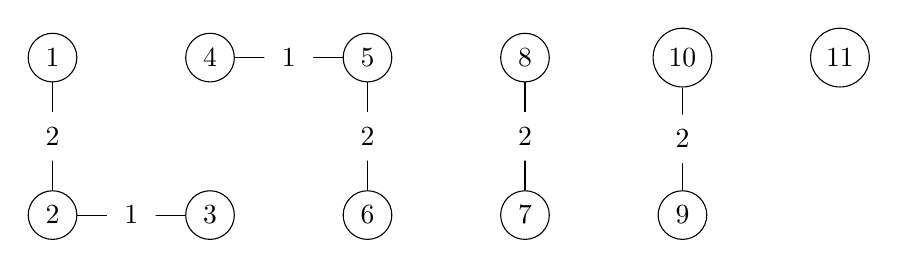
\begin{tikzpicture}

        \begin{scope}[every node/.style={circle,draw}]
          \node (1)  at (0,2)  {1};
          \node (2)  at (0,0)  {2};
          \node (3)  at (2,0)  {3};
          \node (4)  at (2,2)  {4};
          \node (5)  at (4,2)  {5};
          \node (6)  at (4,0)  {6};
          \node (7)  at (6,0)  {7};
          \node (8)  at (6,2)  {8};
          \node (9)  at (8,0)  {9};
          \node (10) at (8,2)  {10};
          \node (11) at (10,2) {11};
        \end{scope}

        \begin{scope}[every node/.style={fill=white,circle}]

          \begin{scope}[every edge/.style={draw}]
            \path (2)  edge node {$1$} (3);
            \path (4)  edge node {$1$} (5);
            \path (1)  edge node {$2$} (2);
            \path (5)  edge node {$2$} (6);
            \path (7)  edge node {$2$} (8);
            \path (9)  edge node {$2$} (10);
          \end{scope}
        \end{scope}

      \end{tikzpicture}
      \caption{[1, 5, 994, 219, 381]}
    \end{center}
  \end{figure}

  \begin{figure}[H]
    \begin{center}
      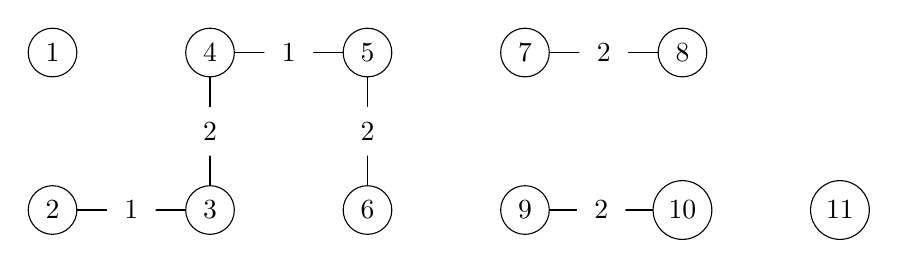
\begin{tikzpicture}

        \begin{scope}[every node/.style={circle,draw}]
          \node (1)  at (0,2)  {1};
          \node (2)  at (0,0)  {2};
          \node (3)  at (2,0)  {3};
          \node (4)  at (2,2)  {4};
          \node (5)  at (4,2)  {5};
          \node (6)  at (4,0)  {6};
          \node (7)  at (6,2)  {7};
          \node (8)  at (8,2)  {8};
          \node (9)  at (6,0)  {9};
          \node (10) at (8,0)  {10};
          \node (11) at (10,0) {11};
        \end{scope}

        \begin{scope}[every node/.style={fill=white,circle}]

          \begin{scope}[every edge/.style={draw}]
            \path (2)  edge node {$1$} (3);
            \path (4)  edge node {$1$} (5);
            \path (3)  edge node {$2$} (4);
            \path (5)  edge node {$2$} (6);
            \path (7)  edge node {$2$} (8);
            \path (9)  edge node {$2$} (10);
          \end{scope}
        \end{scope}

      \end{tikzpicture}
      \caption{[1, 5, 1010, 232, 381]}
    \end{center}
  \end{figure}

  \paragraph{}
  Dans le premier cas, $(\rho_1\rho_2)^2\rho_1$ nous donne ce que nous cherchons. Dans le second, c'est $(\rho_1\rho_2)^4\rho_1$ qui nous donne le résultat

\end{proof}

\paragraph{}
Grâce à ces deux théorèmes, on sait qu'il existe une 2-transposition $g$ dont $\rho_2$ est une extension qui est telle que $ g \in \Gamma_{0,1} = S_7$ et $g \in \Gamma_(0,3,4)$ donc $g \in \Gamma_{0,1} \cap \Gamma_(0,3,4)$ mais $g \notin \Gamma_{0,1,3,4} = <\rho_2>$. Donc $\Gamma_{0,1} \cap \Gamma_{0,3,4} \neq \Gamma_{0,1,3,4}$ donc $\Gamma$ ne satisafait pas la propriété d'intersection et n'est donc pas un C-group. Ce qui conclut la preuve du théorème
